\section{Laboratory Lecture 2: Flip Flops}
\label{sec:FLIP_FLOPS}

The main objective of this lab lecture is to learn about the operation of Flip Flops. In particular, we will discuss how JK flip flops work as well as some of their applications.

\subsection{Introduction}

A flip flop, also known as latch or bistable multivibrator, is a type of circuit that has two states, one of them represents a \textit{one} and the other one a \textit{zero}, i.e. a single bit of data. They are commonly used to store information in digital circuits.\medskip 

Flip flops can be edge-triggered, that is synchronous/clocked, or level triggered, that is asynchronous. In order to control them, we have to apply specific signals to the inputs, following their truth table.\medskip

Some examples of flip flops may include D Flip flops, D Latch Flip flops, SR Flip flops, and JK Flip flops, to name a few. In this practice we are going to work with the latter.

\subsubsection{JK Flip Flops}

Before diving into what a JK Flip Flop is, we will briefly talk about SR Flip Flops, as they are the old and troublesome early version of a JK one.\medskip

SR Flip Flops, also known as SR Latch, are one the most basic sequential logic circuits. They act as a one-bit memory, so a bistable device, that possesses 2 inputs. On the one hand, \textit{SET}, which will output a 1 and is usually labelled \textit{S}, and \textit{RESET}, which will output a 0, and is usually labelled \textit{R}. \medskip

Note than we can also find a clocked, or synchronous variation of the SR Flip Flop. The latter will have an extra input, \textit{CLK} and it will only trigger on the positive edge transitions of the clock.\medskip

Obviously, \textit{SR} stands for "Set-Reset". As we have previously said, the reset input resets the flip flop, that is, it makes the output, Q, go back to its original state of 0. The different input configurations will define the behaviour of the output following this fashion:\medskip


\begin{minipage}{\textwidth}
    \begin{minipage}[b]{0.49\textwidth}
        \centering
        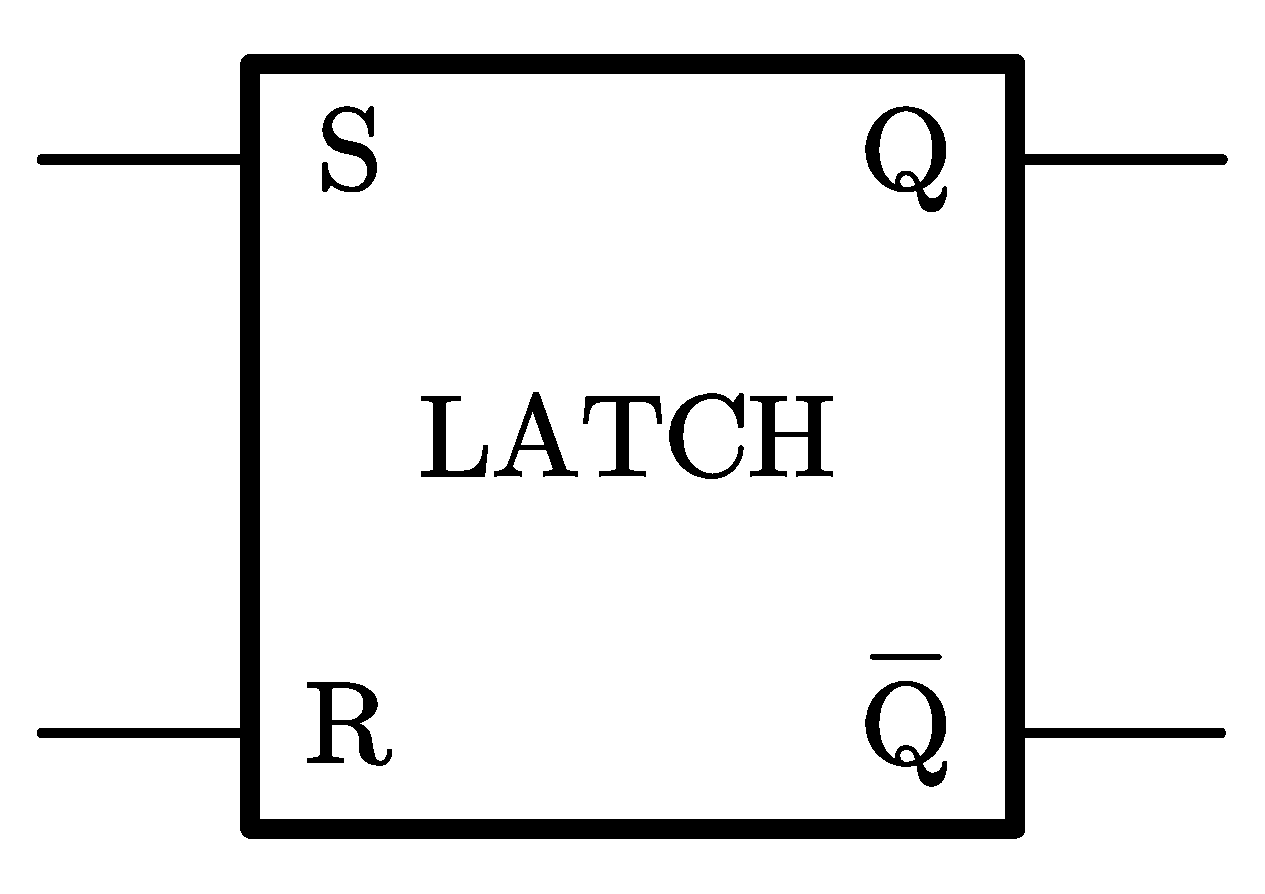
\includegraphics[scale=0.2]{Graphics/Practice 2/GRAPHICS/LOGIC GATES/SR ASYNCH.pdf}
        \captionof{figure}{SR Asynchronous Flip Flop.}
        \label{fig:SR_Asynch}
    \end{minipage}
    \hfill
    \begin{minipage}[b]{0.49\textwidth}
        \centering
             \begin{tabular}[t]{lccc}
                \toprule
                &\textbf{SET}&\textbf{RST}&\textbf{Q}\\
                \midrule
                & 0 & 0 & $Q_0 \text{ No change}$\\
                & 1 & 0 & Q = 1\\
                & 0 & 1 & Q = 0\\
                & 1 & 1 & Invalid\\
                \bottomrule
            \end{tabular}
        \captionof{table}{SR Flip Flop's Truth Table.}
    \end{minipage}
\end{minipage}\textbf{}

\clearpage

As we can deduce from the table, this type of flip flops pose a problem when both the \textit{S} and the \textit{R} inputs are 1, since the output state is invalid and cannot be predicted.\medskip

To solve this problem, we will make use of a \textbf{JK Flip Flop}. JK Flip flops, in a nutshell, solve this problem by having the output toggle when both inputs \textit{J} and \textit{K}, which correspond to the \textit{S} and \textit{R} terminals respectively, are 1. The truth table of this type of flip flop is as follows:\bigskip

\begin{minipage}{\textwidth}
    \begin{minipage}[b]{0.49\textwidth}
        \centering
        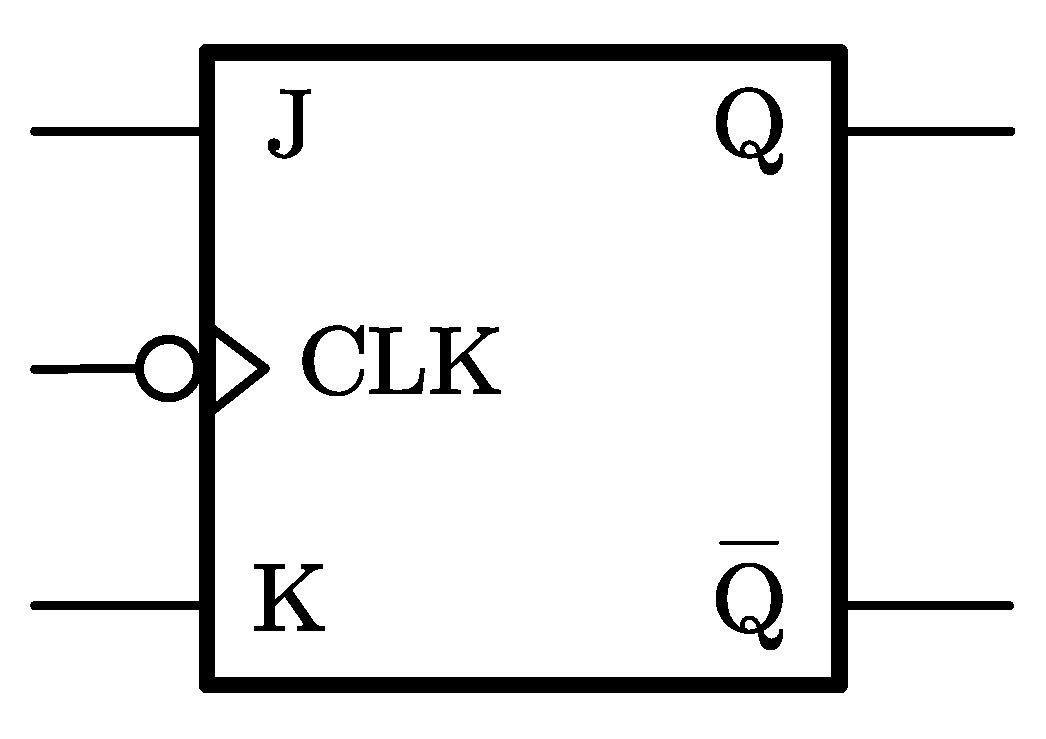
\includegraphics[scale=0.25]{Graphics/Practice 2/GRAPHICS/LOGIC GATES/JK SYNCH.pdf}
        \captionof{figure}{JK Synch. Flip Flop.}
        \label{fig:JK_Synch}
    \end{minipage}
    \hfill
    \begin{minipage}[b]{0.49\textwidth}
        \centering
            \begin{tabular}[t]{lcccc}
                \toprule
                &\textbf{J}&\textbf{K}&\textbf{CLK}&\textbf{Q}\\
                \midrule
                &0&0& $\uparrow$ & $Q_0 \text{ No change}$\\
                &1&0& $\uparrow$ & Q = 1\\
                &0&1& $\uparrow$ & Q = 0\\
                &1&1& $\uparrow$ & $\overline{Q_0} \text{ Toggles}$\\
                \bottomrule
            \end{tabular}
        \captionof{table}{JK's Synch. Truth Table.}
        \label{table:JK_Synch_TT}
    \end{minipage}
\end{minipage}

\vspace{0.5cm}

It is possible to find an asynchronous version of the JK Flip Flop as well. This version has two extra pins, \textit{PRESET} and \textit{CLEAR}, which, if active, will turn the output $Q$ to 0, if the \textit{PRESET} is connected to 1 and the \textit{CLEAR} to 0. Alternatively, they will turn the output $Q$ to 1 if the \textit{PRESET} is connected to 0, and the \textit{CLEAR} to 1. We can visualise this in the following truth table: 

\vspace{0.7cm}

\begin{minipage}{\textwidth}
    \begin{minipage}[b]{0.49\textwidth}
        \centering
        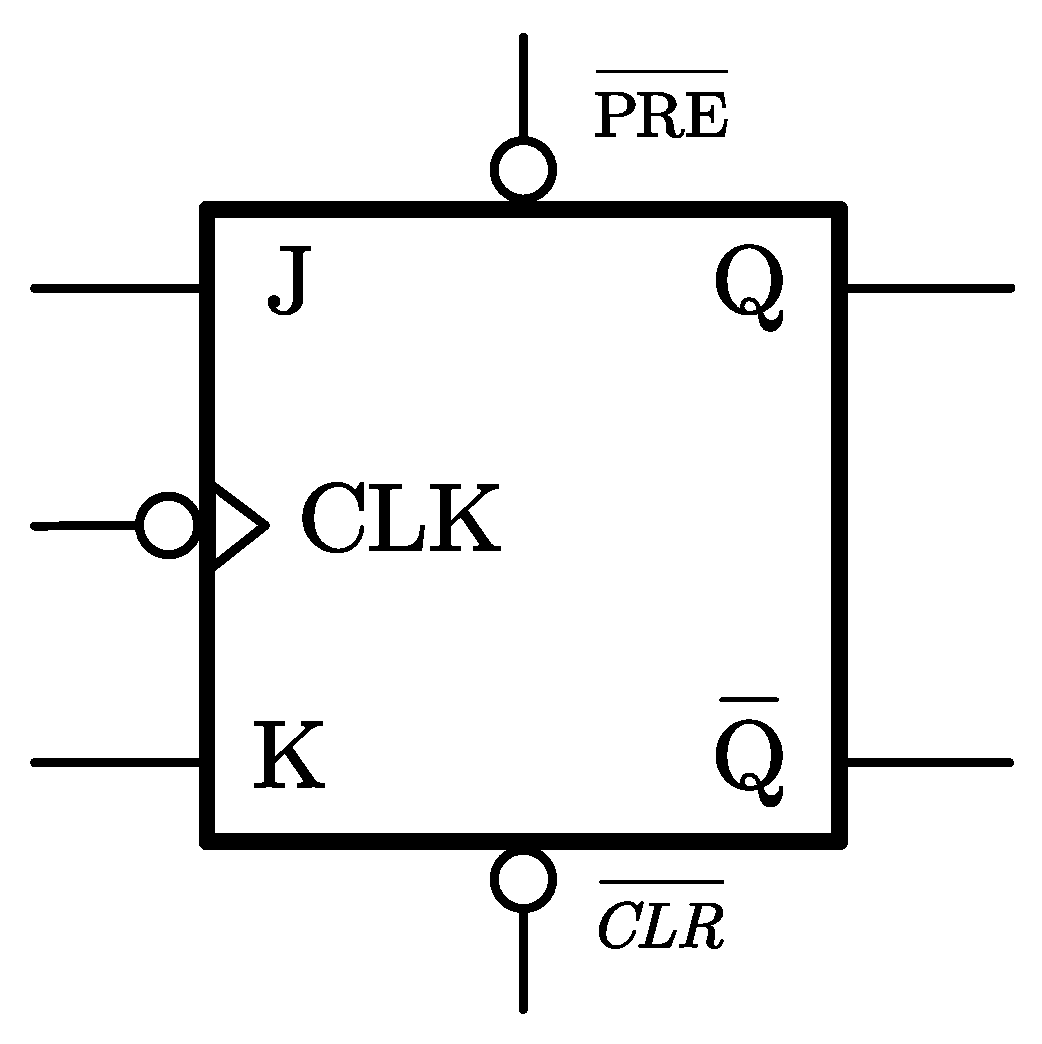
\includegraphics[scale=0.25]{Graphics/Practice 2/GRAPHICS/LOGIC GATES/JK ASYNCH.pdf}
        \captionof{figure}{JK Asynch. Flip Flop.}
        \label{fig:JK_Asynch}
    \end{minipage}
    \hfill
    \begin{minipage}[b]{0.49\textwidth}
        \centering
            \begin{tabular}[t]{lcccccc}
                \toprule
                & \textbf{J} & \textbf{K} & \textbf{CLK} & $\overline{\mathbf{PRE}}$ & $\overline{\mathbf{CLR}}$ & \textbf{Q}\\
                \midrule
                & 0 & 0 & $\downarrow$ & 1 & 1 & $Q_0$\\
                & 1 & 0 & $\downarrow$ & 1 & 1 & 1\\
                & 0 & 1 & $\downarrow$ & 1 & 1 & 0\\
                & 1 & 1 & $\downarrow$ & 1 & 1 & $\overline{Q_0}$\\
                \midrule
                & X & X & X & 0 & 0 & Inv\\
                & X & X & X & 0 & 1 & 1\\
                & X & X & X & 1 & 0 & 0\\
                \bottomrule
            \end{tabular}
        \captionof{table}{JK's Asynch. Truth Table.}
        \label{table:JK_Asynch_TT}
    \end{minipage}
\end{minipage}\textbf{}

\newpage

Now that we have established the basics, we will move on to completing the laboratory session.

\subsection{JK Synchronous Flip Flop}

\subsubsection{Asynchronous \textit{PRE} and \textit{CLR} effect on Q}

In order to complete this part, we will make use of the program Proteus, as per usual. We will simply follow Table \ref{table:JK_Asynch_TT} in order to check the output when \textit{PRE} and \textit{CLR} change.

\begin{figure}[H]
    \centering
    
    \ifnum\value{ANIMATION}=1 {
        \animategraphics[controls,loop,scale=1.4]{1}{Graphics/Practice 2/GRAPHICS/ANIMATION/JK ASYNCH/F}{0}{2}
    } 
    \else {
        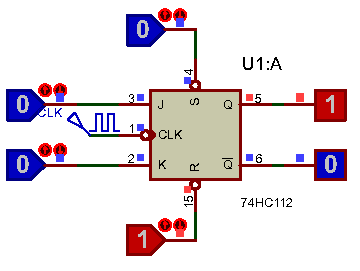
\includegraphics[scale=1.4]{Graphics/Practice 2/GRAPHICS/ANIMATION/JK ASYNCH/F1.PDF}
    }\fi
    
    \caption{Proteus assembly.}
    \label{fig:PROTEUS_JK_ASYNCH}
\end{figure}

In the simulation, we can not only see that the output, $Q$, is correct, but that it also does not depend on the values of \textit{J}, \textit{K}, and \textit{CLK}. 

\subsubsection{Synchronous \textit{J} and \textit{K} effect on Q}

For this part, as we are working with a Synchronous circuit, both \textit{PRE} and \textit{CLR} have to be tied to their inactive state, in this case, since they are active low, we will tie them to 1.

Again, we have to check that the circuit behaves as expected, that it, that it follows Table \ref{table:JK_Synch_TT}

\newpage

To achieve this, we will use Proteus once more.

\begin{figure}[H]
    \centering
    
    \ifnum\value{ANIMATION}=1 {
        \animategraphics[controls,loop,scale=1.4]{1}{Graphics/Practice 2/GRAPHICS/ANIMATION/JK SYNCH/F}{0}{5}
    } 
    \else {
        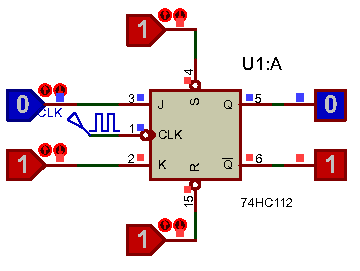
\includegraphics[scale=1.4]{Graphics/Practice 2/GRAPHICS/ANIMATION/JK SYNCH/F2.PDF}
    }\fi
    
    \caption{Proteus assembly.}
    \label{fig:PROTEUS_JK_SYNCH}
\end{figure}

As we can see, the circuit behaves as expected.


\subsection{T Flip Flop from JK Flip Flop}

In this exercise we are asked to create a T Flip Flop using a JK one. To do this we have to take Table \ref{table:JK_Synch_TT} into account, as it clearly states that when both inputs, \textit{J} and \textit{K} are tied to 1, and a falling edge of the clock occurs -in the case of a 74HC112-, the output toggles, which is precisely what we aim to obtain.


\begin{figure}[H]
    \centering
    
    \ifnum\value{ANIMATION}=1 {
        \animategraphics[controls,loop,scale=1.4]{2}{Graphics/Practice 2/GRAPHICS/ANIMATION/T/F}{0}{1}
    } 
    \else {
        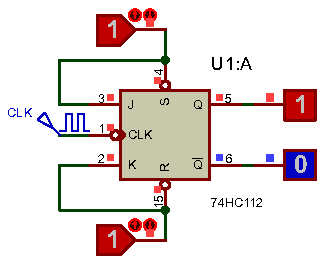
\includegraphics[scale=1.4]{Graphics/Practice 2/GRAPHICS/ANIMATION/T/F1.PDF}
    }\fi
    
    \caption{Proteus assembly.}
    \label{fig:PROTEUS_T}
\end{figure}

\clearpage

One of the most important applications of this type of gate is to build a frequency divider. Since we are using a 74HC112 as a T Flip Flop, if we apply a \textit{CLK} signal with a duty cycle of $50\%$ to the clock input, the output $Q$ will toggle every time a falling edge occurs, that is, every full cycle, effectively dividing the input frequency by 2. We can visualise this in the following timing diagram: \medskip

\begin{figure}[H]
    \centering
    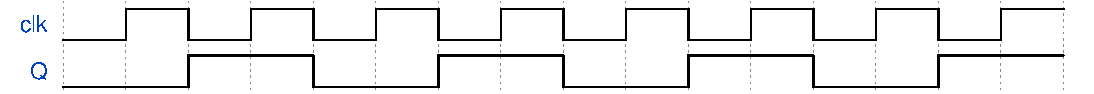
\includegraphics[scale = 0.73]{Graphics/Practice 2/GRAPHICS/TIMING/EX2.pdf}
    \caption{Timing diagram of a 2-bit frequency divider.}
    \label{fig:timing_1}
\end{figure}

\subsection{T Flip Flop Asynchronous counter}

Now that we have established how to build a frequency divider, we will focus on its applications. In particular, we will build a binary counter, which will be fed to a BCD to 7 segment display decoder, so as to help us visualise the output.\medskip

In Figure \ref{fig:timing_1}, we can already see the the behaviour that we are aiming for. In the first division, the \textit{Q} and the \textit{clk} signals have a logic level of 0, or 00 in binary. This value turns into a 01 in the second division, 10, in the third, and finally 11 in the fourth. Translating these numbers into decimal yields 0, 1, 2, 3, so we can say that Figure \ref{fig:timing_1} represents a 2 bit binary counter.\medskip

In order to be able to display numbers up to 7, we will need a 3 bit binary counter. Building it is just a matter of concatenating 2 T Flips Flops following this fashion:

\begin{figure}[H]
    \centering
    
    \ifnum\value{ANIMATION}=1 {
        \animategraphics[controls,loop,scale=0.85]{2}{Graphics/Practice 2/GRAPHICS/ANIMATION/7_SEG/F}{0}{7}
    } 
    \else {
        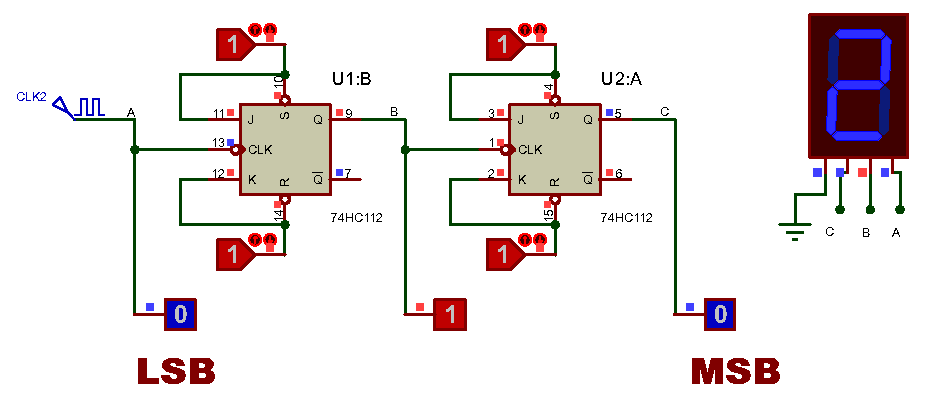
\includegraphics[scale=0.85]{Graphics/Practice 2/GRAPHICS/ANIMATION/7_SEG/F2.PDF}
    }\fi
    
    \caption{Proteus assembly.}
    \label{fig:PROTEUS_7_SEG}
\end{figure}

\clearpage

If we look at the output signals with a logic analyser, we will see the following:\medskip

\begin{figure}[H]
    \centering
    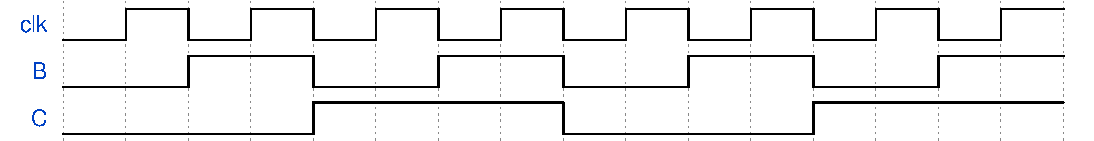
\includegraphics[scale = 0.73]{Graphics/Practice 2/GRAPHICS/TIMING/EX3.pdf}
    \caption{Timing diagram of a 3-bit frequency divider.}
    \label{fig:timing_2}
\end{figure}

The only problem that this configuration poses, is that a small glitch is produced at the output due to the propagation time of the \textit{CLK} signals, as the output of the first T Flip Flop is fed into the input of the next one and so on.\medskip 

One possible solution would be to add a capacitor connected to ground to each of the 3 outputs, in order to smooth out the peak and make the transition more visually appealing and less prone to error.

\clearpage
